\chapter{Hello World} 
I've read lots of articles from hundreds of websites and blogs which taught me much knowledge. I really appreciated these authors which gave contributions to the world and other peoples. So that's why I will write some articles for sharing my experiences and as in return.

Although reading is the best time of mine, there were lots of plains reading online. Commercial blogs always have lots of ads which try its best to catch you attention; Many page elements like the social button, the recent and related posts\sidenote{I do believe the sidebars of "Wordpress" will attract the reader's attention.}, the comments, even the categeries and tags of the blog, or something else, all they were disturbing you and making you easy to uncomplete this article; And some blogs, which really includes valuable information, but due to the bad typesetting, you even might lost patients to finish it.  

So I almost always save articles I like to Pocket\sidenote{Pocket is my best favorite App, Please see: https://getpocket.com/}, which is my most favorite App. Pocket will remove all the other useless elements but the content of the article itself and display in a beautiful view. I love it so much and I was be told that I was their top 5 readers for twice in the last two years. Another way I liked is the Safari's "Reader view", which has the similar function as Pocket.

The world's most beautiful typesetting is Latex, which is the most popular solution in the publishing industry. Thousands of books were written by Latex. But using Latex online is difficult. Fortunately there were some solutions which could help working with Wordpress. There I will introduce my way and the tools.
    
Basically, the most element in an article (or book) are sections, tables, figures, sidenotes and footnotes. These all are used in this blog. Let me explain how.


\section{Figures}
The most important element in an article is figure(of curse you might have different opinion) - especially in Computer Graphics filed. The image should be a vector image which can be scaled arbitrarily. I choose Inkscape\sidenote{Inkscape: https://inkscape.org/en/} to draw the image and saved it as svg format. The img tag of html can use it as a source file. 

In order to avoid inputting the html code and css style every time, I used the Wordpress's add\_shortcode function to do it for me. So the code will be very simple. Like:

\begin{lstlisting}[frame=single,breaklines=true]
[figure index=1 src='/wp-content/uploads/file.svg']This is an example of figures[/figure]
\end{lstlisting}

will generates the figure looks like this:

\begin{figure}
	\includegraphics{graphics/demo}
	\caption{This is an example of figures}
\end{figure}

Bad thing is the svg file is so large, the above image has 2.1MB. But since you will never visit this blog like twitter, So I think it's acceptable. After all the most important thing should be to make the feeling of reading better, so you could have more chance to finish it.   

For some small figures I will put them on the right side, like this
\begin{marginfigure}
	\includegraphics{graphics/Einstein}
	\caption{This is an example of figures}
\end{marginfigure}

\subsection{Equation Graph}

For the math equation graph, it's hard to draw it in inkscape. If you are using Mac OS there is a perfect build-in tool names 'Grapher'\sidenote{Grapher: https://en.wikipedia.org/wiki/Grapher}. Its perfect for drawing math equations but unfortunately it can only export as tiff, jpeg, pdf and eps format. Only jpeg and tiff can be used in 'img' tag. 'jpeg' is low quality and 'tiff' file is too large(far than svg). So I used a stupid method that use inkscape convert pdf file to svg. Following is an example of Bassel Function:

\begin{figure}
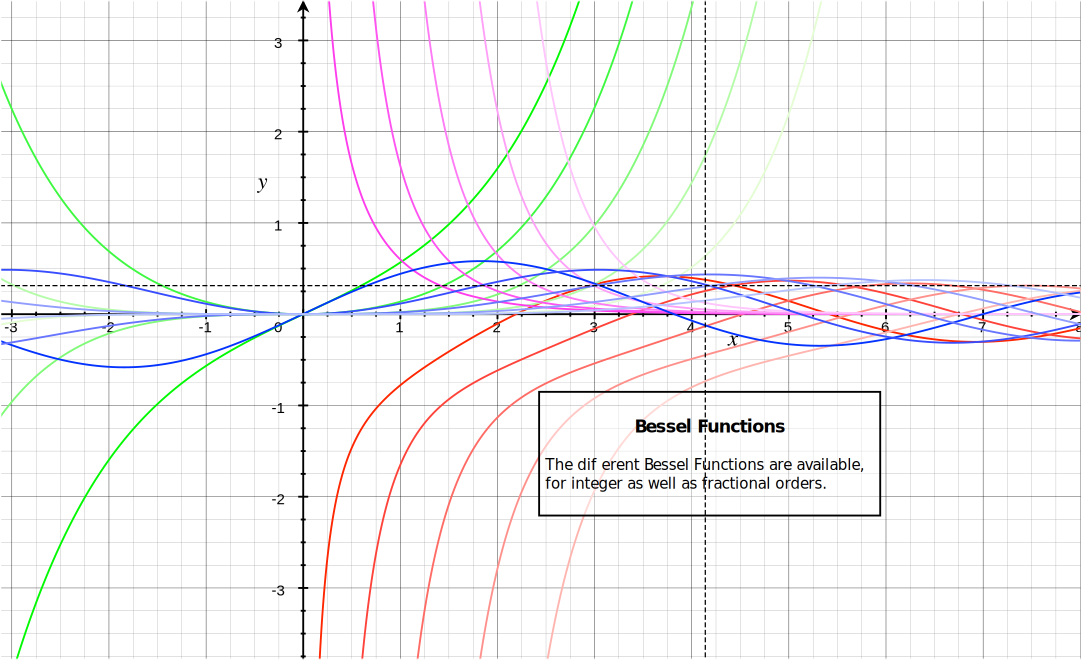
\includegraphics{graphics/Bessel-Functions}	
\caption{This is an example of Bessel Functions[}
\end{figure}

There is a problem: the fontsize of the text in the image isn't match the size of the article(You might have seen in the above picture). Because image just be scaled to a fixed rectangle. The only thing you can do is to make sure the actual size of the draw area in 'Grapher' close the size the page used. Otherwise you can draw figure in latex directly.


\section{Tables}
The second thing should be Tables. Both figures and tables in an article can explain more than the text. Most importantly save the time the reader understanding the knowledge. Rather than take 5 minutes to read the text, the reader can know what the paragraph said at once.

In a Web environment you can use html table, tr and td tags to edit a table. But this method can only be used for webpage. Actually I hope the most content of an article can be edited in my local Latex editor. So, you might have figured out, I still choose Latex way.

But Table is more difficult than figures. For figures there just is an simple image. All the process of creating the image is offline. I just need to use a img tag. But HTML can not know what's Latex. Also, I can't render the table as a svg file like the figure. Because a table contains lots of texts, which need to make a adjust to adapter  the size of the article content(the same problem mentioned above). So I need another way.

Finally I choose QuickLatex\sidenote{QuickLatex: http://www.quicklatex.com/}, which is a plugin for Wordpress. It can render the Latex table code into a svg file and load it automatically. So I can put the Latex code into the Wordpress Editor. Of course there are few changed has to be made. You might check the QuichLatex site for detials, or you could leave comment if you need.     

The following code:
\begin{fullwidth}
\begin{lstlisting}[frame=single,breaklines=true]
<p style="text-align:center">
[latex mode=1]
\begin{table}
    \begin{tabular}{|l|l|}
    \hline
    real time           & Physically Based                               \\ \hline
    Real-Time Rendering & Physically Based Rendering                     \\ \hline
    Real-Time Shadows   & Advanced Global Illumination                   \\ \hline
    GPU Pro 5           & Realistic Image Synthesis Using Photon Mapping \\ \hline
    \end{tabular}
\caption{Some Computer Graphics books}
\end{table}
[/latex]
</p>
\end{lstlisting}
\end{fullwidth}

will looks like this:

\begin{table}
    \begin{tabular}{|l|l|}
    \hline
    real time           & Physically Based                               \\ \hline
    Real-Time Rendering & Physically Based Rendering                     \\ \hline
    Real-Time Shadows   & Advanced Global Illumination                   \\ \hline
    GPU Pro 5           & Realistic Image Synthesis- Photon Mapping \\ \hline
    \end{tabular}
\caption{Some Computer Graphics books}
\end{table}

\section{sidenotes}
Sidenotes is my best favorate part. In "A TUFTE-STYLE BOOK"\sidenote{tufte-latex: https://www.ctan.org/pkg/tufte-latex?lang=en}, the author treat sidenode as a very import role and I absolutely agree!

I want to explain why. Traditionally, the author might put some closer but simple elaboration or some related concept or resources on the side position, which might beyond the range of the paragraph but can make the concept easier to understand. Some authors would like treat them as a footnoote. But footnote will make the reader have to move their sight to another place, and the reader\citet{b:implicit-surfaces} has to take times move back to where the place \citet{b:rts} stopped. Even worse, This process might interrupt the reader's train of \citet{b:pbrt} thought.  

So this reason makes the sidenote more important. You might have noticed that I even removed the whole sidebar of Wordpress, and leaves this place entirely for sidenote.\sidenote{My name is 'sidenote'. I can explain more. Giving more information, showing a figure, or just a reference, etc. You will like me very much.} 

\section{footnotes}

Of cause footnote still has its usage and role. Basically it's only for reference, a link, book or something like this. The footnotes located on the bottom of the article. You also could click the number tag\sidenote{This is a test for footnote} go to their directly.

\section{End}
I hope you will like this!